\documentclass[a4paper,10pt,twoside,openany]{book}

\usepackage[lang=hebrew]{maths}
\usepackage{hebrewdoc}
\usepackage{stylish}
\usepackage{lipsum}
\let\bs\blacksquare

%TIKZSETS
\tikzset{
    labl/.style={anchor=south, rotate=90, inner sep=.5mm}
}

\title{סיכומי הרצאות בתורת מורס \\ \large{אביב 2021, הטכניון}}
\author{הרצאותיו של מיכאל חנבסקי \\ \large סוכמו על ידי אלעד צורני}
\date{\today}

\begin{document}
\frontmatter
\frontpage{cover}{0.8\textwidth}{חלקים שקולים הומוטופית של הטורוס.}
\tableofcontents
\countlectures
\newpage

\chapter*{הקדמה}
\addcontentsline{toc}{chapter}{הקדמה} \markboth{הקדמה}{}

\section*{הבהרה}
\addcontentsline{toc}{section}{הבהרה} %\markboth{Technicalities}{}

סיכומי הרצאות אלו אינם רשמיים ולכן אין
\emph{כל הבטחה}
כי החומר המוקלד הינו בהתאמה כלשהי עם דרישות הקורס, או שהינו חסר טעויות.
\\
להיפך, ודאי ישנן טעויות בסיכום! אעריך אם הערות ותיקונים ישלחו אלי בכתובת דוא"ל
\textenglish{\href{mailto:tzorani.elad@gmail.com}{tzorani.elad@gmail.com}}.\\
אלעד צורני.

\section*{ספרות מומלצת.}
\addcontentsline{toc}{section}{ספרות מומלצת} %\markboth{Course Literature}{}

הספרות המומלצת עבור הקורס הינה כדלהלן.

\begin{english}
\begin{description}
\item[J. Milnor:] Morse Theory

\item[A. Banyaga, D. Hurtubise:] Lectures on Morse Homology

\item[M. Audin, M. Damian:] Morse Theory and Floer Homology
\end{description}
\end{english}

\section*{ציון}
הציון בקורס ינתן עבור מבחן בית שעשוי (ועשוי לא) לכלול מעבר בעל פה על הפתרונות.

\section*{דרישות קדם}

דרישת הקדם לקורס היא יריעות דיפרנציאביליות. היכרות עם טופולוגיה אלגברית מועילה אך אינה חיונית.

\mainmatter

\chapter{מבוא}
\section{מוטיבציה}

\begin{example}

\begin{figure}
\centering
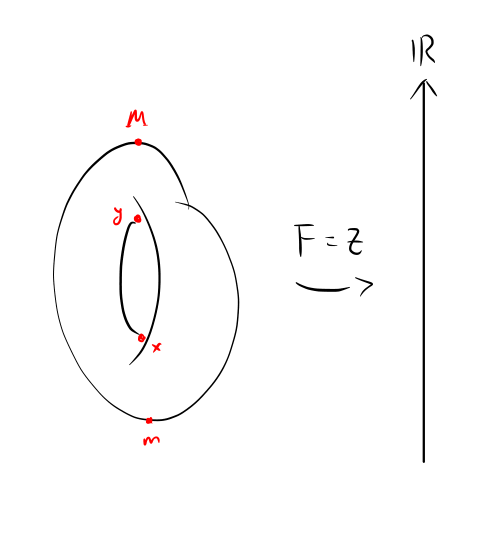
\includegraphics[scale=0.5]{sources/1.1}
\caption{העתקת גובה מהטורוס, והנקודות הקריטיות שלה.}
\label{1.1}
\end{figure}

באיור
\ref{1.1}
הנקודות המסומנות מאדום הן הנקודות הקריטיות של
$F$.
נסמן
\[\text{.} \mbb{T}^a \ceq \set{p \in \mbb{T}^2}{F\prs{p} < a}\]
\begin{itemize}
\item עבור
$a \leq F\prs{m}$
נקבל
$\mbb{T}^a = \ns$.
\item עבור
$F\prs{m} < a \leq F\prs{x}$
נקבל
$\mbb{T}^a \cong D^2$.
ראו איור
\ref{1.2}.

\begin{figure}
\centering
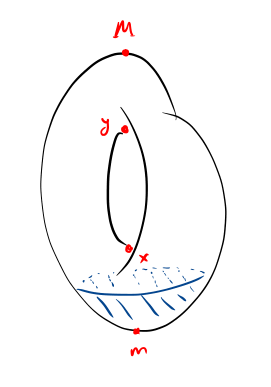
\includegraphics[scale=0.5]{sources/1.2}
\caption{חתך של הטורוס שדיפאומורפי ל־%
$D^2$.}
\label{1.2}
\end{figure}

\item עבור
$F\prs{x} < a \leq F\prs{y}$
נקבל
$\mbb{T}^a \cong S^1 \times \prs{0,1}$.
ראו איור

\begin{figure}
\centering
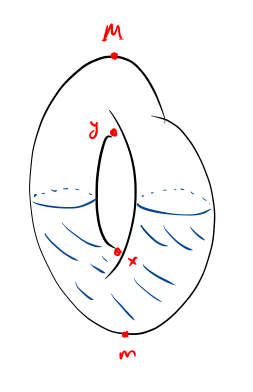
\includegraphics[scale=0.5]{sources/1.3}
\caption{חתך של הטורוס שדיפאומורפי ל־%
$S^1 \times \prs{0,1}$.}
\label{1.3}
\end{figure}

\item
עבור
$F\prs{y} < a \leq F\prs{M}$
נקבל
$\mbb{T}^a \cong \mbb{T}^2 \setminus D^2$.
\item עבור
$F\prs{M} < a$
נקבל
$\mbb{T}^a = \mbb{T}^2$.
\end{itemize}

\begin{corollary}
אם ב־%
$\left[ a, b \right)$
אין ערכים קריטיים אז
$\mbb{T}^a \cong \mbb{T}^b$.
\end{corollary}

נשאל איך משתנה הטופולוגיה במעבר בנקודות הקריטיות.
\begin{itemize}
\item במעבר דרך
$F\prs{m}$
יש הוספת דיסק.
\item כאשר
$a = x-\eps$
עבור
$\eps$
מספיק קטן, קו הגובה יראה באיור
\ref{1.4}
אם נדביק את
$\mbb{T}^a$
על פס כבאיור
\ref{1.5}
נקבל יריעה דיפאומורפית ל־%
$\mbb{T}^x+\eps$.

\begin{figure}
\centering
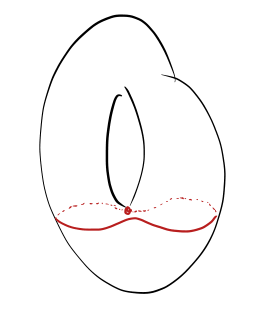
\includegraphics[scale=0.5]{sources/1.4}
\caption{קו גובה על הטורוס קרוב לנקודת אוכף.}
\label{1.4}
\end{figure}

\begin{figure}
\centering
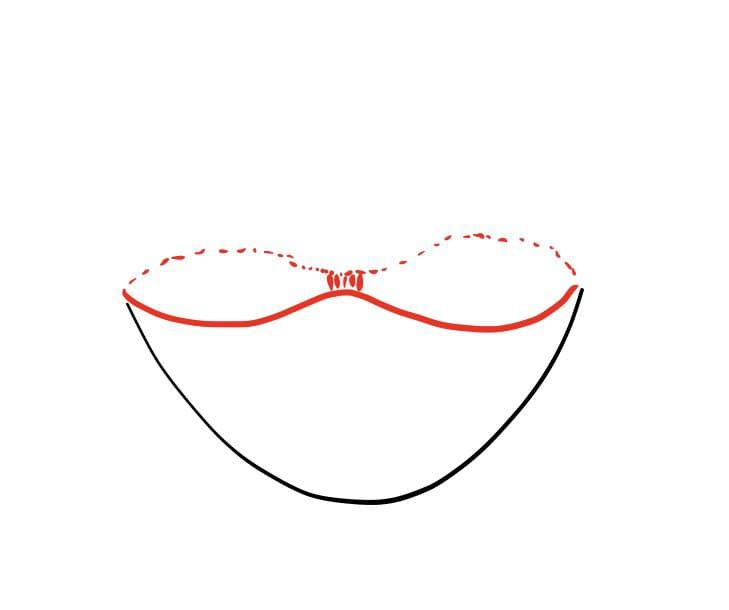
\includegraphics[scale=0.3]{sources/1.5}
\caption{הדבקת חתך של הטורוס קרוב לנקודת אוכף.}
\label{1.5}
\end{figure}

\item כאשר
$a = y+\eps$
עבור
$\eps$
מספיק קטן נקבל כי
$\mbb{T}^a$
כבאיור
\ref{1.6}.
אם נדביק את העיגולים באידומים באיור על פס כבאיור
\ref{1.7}
נקבל יריעה דיפאומורפית ל־%
$\mbb{T}^a$
עבור
$a = y + \eps$.

\begin{figure}
\centering
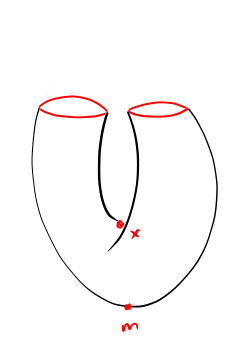
\includegraphics[scale=0.5]{sources/1.6}
\caption{חתך של הטורוס קרוב לנקודת אוכף.}
\label{1.6}
\end{figure}

\begin{figure}
\centering
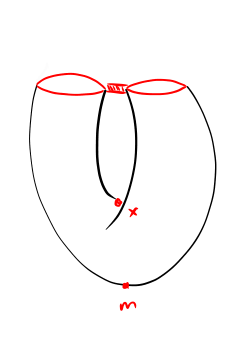
\includegraphics[scale=0.5]{sources/1.7}
\caption{הדבקת חתך של הטורוס קרוב לנקודת אוכף.}
\label{1.7}
\end{figure}

\item במעבר דרך
$F\prs{M}$
יש הדבקה של
$D^2$
לשפה של
$\mbb{T}^{F\prs{M} - \eps}$.
\end{itemize}

\end{example}

ראינו שבמקרה של הטורוס יש לנקודות הקריטיות חשיבות רבה במבנה של היריעה. אנחנו נראה בקורס שאפשר לשחזר אינווריאנטים כמו ההומולוגיה של יריעה בעזרת הבנה של הנקודות הקריטיות.
במקרה של הטורוס, מתקיים
\begin{align*}
H_0\prs{\mbb{T}^2, \mbb{Z}} &= \mbb{Z} \cong \mbb{Z}\trs{m} \\
H_1\prs{\mbb{T}^2, \mbb{Z}} &= \mbb{Z}^2 \cong \mbb{Z}\trs{x,y} \\
\text{.} H_2\prs{\mbb{T}^2, \mbb{Z}} &= \mbb{Z} \cong \mbb{Z}\trs{M}
\end{align*}
נדבר על דרך כללית להבין הומולוגיה וקוהומולוגיה של יריעות בעזרת נקודות קריטיות. נדבר על דואליות פואנקרה, על מבנה של כפל בקוהומולוגיה, על העתקות טבעיות, על מקדמים בחוגים שונים, וכו'.

בין היתרונות של תורת מורס הם שהיא נותנת את ה(קו)הומולוגיות הסטנדרטיות על יריעות, ושהיא עובדת עבור אוביקטים אינסוף־מימדיים.

\begin{example}[\textenglish{Path-Space}]
תהי
$M$
יריעה רימנית ויהי
\[\text{.} \mcal{P}\prs{x,y} = \set{\gamma \colon \brs{0,1} \to M}{\substack{\gamma\prs{0} = x \\ \gamma\prs{1} = y}}\]
על מרחב זה אפשר להגדיר כל מני פונקציות, למשל
\begin{align*}
\len \colon \mcal{P}\prs{x,y} &\to \mbb{R} \\
\text{.} \gamma &\mapsto \int_0^1 \norm{\dot{\gamma}} \diff s
\end{align*}

אפשר לנסות לעבוד עם תורת מורס על פונקציה כזאת ולהבין את המרחב
$\mcal{P}\prs{x,y}$
בעזרת הנקודות הקריטיות של
$\len$.
במקרה הזה, הנקודות הקריטיות הן קווים גיאודזיים. הן אינן מבודדות וקשה להסיק דברים על המרחב.

במקרה של
\[ \phi\prs{\gamma} = \int_0^1 \norm{\dot{\gamma}}^2 \diff s\]
הנקודות הקריטיות יהיו קווים גיאודזים עם מהירות קבועה. אז הנקודות הקריטיות בדרך כלל יהיו מבודדות, ויהיה אפשר להשתמש בתורת מורס.
\end{example}

\section{נקודות קריטיות}

במהלך הקורס נניח כי כל המבנים חלקים.
התוצאות נכונות באופן כללי יותר עבור יריעות
$\mcal{C}^2$,
שדות וקטוריים
$\mcal{C}^1$
ופונקציות דיפרנציאביליות
$\mcal{C}^2$.

\begin{definition}[נקודה קריטית]
תהי
$F \colon M \to N$
העתקה חלקה בין יריעות חלקות.
נקודה
$p \in M$
נקראת
\emph{קריטית}
אם
$D f_p \colon T_p M \to T_{f\prs{p}} N$
אינה על.
\end{definition}

\begin{remark}
\begin{enumerate}
\item במסגרת הקורס נדון בפונקציות
$F \colon M \to \mbb{R}$.
אז
$p \in M$
נקודה קריטית אם ורק אם
\[D F_p \colon T_p M \to T_{f\prs{p}} \mbb{R}\]
אינה על.
כיוון ש־%
$T_{f\prs{p}} \mbb{R}$
מרחב לינארי חד־מימדי זה שקול לכך שמתקיים
$D F_p = 0$.

\item
ניתן לזהות
$T_{f\prs{p}}\mbb{R} \cong \mbb{R}$
בדרך קנונית. נגדיר את ההרכבה של העתקה זאת על
$D F_p$
להיות
\emph{הנגזרת החיצונית של
$F$
בנקודה
$p$}.
נראה זאת בדיאגרמה הבאה.
\[
\begin{tikzcd}
T_p M \arrow[r, "D F_p"] \arrow[dr, dotted, swap, "\diff F_p"] & T_{f\prs{p}}\prs{\mbb{R}} \arrow[d, "\sim" labl] \\ & \mbb{R}
\end{tikzcd}
\]
נקבל כי
$p \in M$
נקודה קריטית אם ורק אם
$\diff F_p = 0$.

זאת תהיה ההגדרה שנעבוד איתה במשך רוב הקורס.

\item אם נפתח את ההגדרה של הנגזרת החיצונית נקבל כי
$p \in M$
נקודה קריטית אם ורק אם
$\frac{\del F}{\del v}\prs{0} \ceq \diff F_p\prs{v} = 0$
לכל
$v \in T_p M$.
מכך נסיק כי נקודות מינימום ומקסימום הן נקודות קריטיות.
כמו כן, ניתן לראות מכך כי נקודות אוכף הן נקודות קריטיות.
\end{enumerate}
\end{remark}

\begin{example}
יהי
$M \subseteq \mbb{R}^3$
משטח ותהי
$F \colon M \to \mbb{R}$
פונקציית גובה.
נגדיר
\begin{align*}
f \colon \mbb{R}^3 &\to \mbb{R} \\
\pmat{x\\y\\z} &\mapsto z
\end{align*}
ואז
$F = \rest{f}{M}$.

אז
$\diff f = \diff z$
ומתקיים
\[\text{.} \diff F_p = \rest{\diff f}{T_p M} = \rest{\diff z}{T_p M}\]
אז
\begin{align*}
\diff F_p = 0 &\iff \rest{\diff z}{T_p M} = 0
\\&\iff T_p M = \ker\prs{\diff z}
\\&\iff T_p M \parallel \spn\prs{x,y} \\
\\&\iff T_p M = \pmat{0 \\ 0 \\ 1}^\perp \\
\\\text{.} \hphantom{\diff F_p = 0} T_p M^\perp = \span\set{\pmat{0\\0\\1}}
\end{align*}
בדוגמה באיור
\ref{1.1}
נקבל שהנקודות הקריטיות הן בדיוק אלו המסומנות. אלו הנקודות בהן הנורמל למישור הוא כפולה של
$z$.
\end{example}

כעת נרצה לעבוד עם שדות וקטוריים במקום נגזרות חיצוניות. במקרה זה אפשר להסתכל על זרימות לאורך שדה ועל הומוטופיות, מה שחסר במקרה של הנגזרת חהיצונית. נתחיל בהגדרה של גרדיאנט ובקשר שלו לנגזרת החיצונית.

\begin{definition}[גרדיאנט]
תהי
$\prs{M,g}$
יריעה רימנית.
ותהי
$F \colon M \to \mbb{R}$
פונקציה חלקה.
לכל
$p \in M$,
$g$
משרה איזומורפיזם
\begin{align*}
g \colon T_p M &\riso T_p^* M \\
\text{.} \hphantom{lalala} v &\mapsto g\prs{v, \cdot}
\end{align*}

\emph{הגרדיאנט של
$F$}
שנסמנו
$\nabla_g F$
או בדרך כלל
$\nabla F$
מוגדר להיות השדה היחיד המקיים
\begin{align*}
\text{.} g\prs{\nabla F, \cdot} = \diff F
\end{align*}
\end{definition}

\begin{remark}
הגרדיאנט
$\nabla F$
תלוי בבחירת
$g$!
\end{remark}

\begin{remark}
מתקיים
\[\diff F_p = 0 \iff \nabla_g F_{\prs{p}} = 0\]
וזה בלתי־תלוי בבחירת
$g$.

נקבל מכך כי
$p \in M$
נקודה קריטית עבור
$F$
אם ורק אם
$\nabla F_{\prs{p}} = 0$.
\end{remark}

\begin{proposition}
תהי
$F \colon M \to \mbb{R}$
ויהיו
$a < b$
כך שקיים
$\eps > 0$
עבורו הקטע
$\prs{a-\eps, b}$
אינו מכיל ערכים קריטיים.
לדוגמא ראו איור
\ref{1.8}.

\begin{figure}
\centering
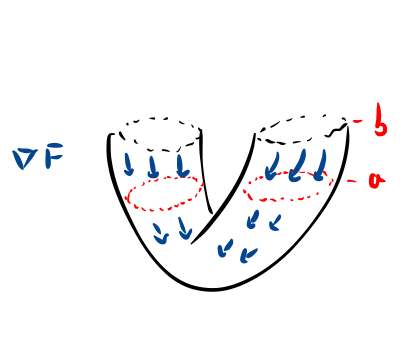
\includegraphics[scale=0.5]{sources/1.8}
\caption{זרימה על הטורוס לאורך הגרדיאנט.}
\label{1.8}
\end{figure}

אז יש דיפאומורפיזם
$M^a \cong M^b$.
\end{proposition}

\begin{proof}
נרצה לנרמל את הגרדיאנט כדי שמהירות הזרימה תהיה אחידה. כדי לא לחלק באפס, נאפס את השדה מתחת לגובה
$a-\eps$.

תהי
$g$
מטריקה רימנית על
$M$.
נסמן
$X = -\nabla_g F$.
עבור
$p \in M^b$
נסתכל על
$\frac{X_p}{\norm{X_p}^2}$.
זה מגדיר שדה וקטורי שלאורכו
$F$
יורדת במהירות
$1$.%
\footnote{
גיאומטרית,
$\frac{X}{\norm{X}}$
וקטור יחידה שמצביע בכיוון בו
$F$
עולה הכי מהר, ומהירות העליה לאורכו היא
$\norm{X}$. לכן כדי שהמהירות תהיה קבועה חלקנו ב־%
$\norm{X_p}^2$.}
%TODO footnote ruler to the right

תהי
\begin{align*}
\rho \colon \prs{-\infty, b} \to \mbb{R}
\end{align*}
חלקה עבורה
\begin{align*}
\rest{\rho}{-\infty, a-\eps} &\equiv 0 \\
\rest{\rho}{\prs{a,b}} &\equiv 1 \\
\text{.} \hphantom{lala} \rho' \geq 0
\end{align*}
אז נוכל להגדיר
\[X' = \frac{\rho X_p}{\norm{X_p}^2}\]
לכל
$F\prs{p} \in \prs{a-\eps, b}$
ונרחיב את
$X'$
מתחת לגובה
$a-\eps$
עם אפסים.
למד"ר המוגדרת על ידי
$X'$
יש פתרונות לכל זמן
$t \geq 0$.

תהי
$\phi_t \colon M^b \to M^b$
זרימה של
$X'$.
אז
$\phi_{b-a} \colon M^b \riso M^a$
דיפאומורפיזם.
\end{proof}

\section{הדבקת ידיות}

\subsection{פונקציות מורס}

נרצה כעת להבין מה קורה איך היריעות
$M^a, M^b$
משתנות כאשר עברו מ־%
$a$
ל־%
$b$
דרך נקודה קריטית.
זה דבר מסובך מאוד באופן כללי ולכן ניאלץ לצמצם את הדיון לנקודות קריטיות שאינן מנוונות.

\begin{definition}[הסיאן]
תהי
$M$
יריעה רימנית ותהי
$F \colon M \to \mbb{R}$
חלקה.
לכל
$p \in $
נגדיר
\[\mrm{Hess}_p\prs{F} \colon T_p M \times T_p M \to \mbb{R}\]
על ידי
$\mrm{Hess}\prs{F} = \nabla \diff F$
כאשר
$\nabla$
הוא ה־%
\href{https://en.wikipedia.org/wiki/Levi-Civita_connection}{\textenglish{Levi-Civita Connection}}.

הגדרה מפורשת יותר היא
\begin{align*}
\mrm{Hess}_p\prs{F} \prs{X_p,Y_p} &= \trs{\nabla_X \mrm{grad}\prs{F_p}, Y_p}
\\&= L_X L_Y \prs{F} - \diff F_p\prs{\nabla_X Y}
\end{align*}
עבור שני שדות וקטוריים
$X,Y$
שמוגדרים סביב
$p$.
\end{definition}

\begin{remark}
הבחירה של ההסיאן תלויה בבחירה של המטריקה הרימנית.

במקרה הפרטי ש־%
$p$
נקודה קריטית מתקיים
$\diff F_p = 0$
ואז
\[\text{.} \mrm{Hess}_p\prs{F}\prs{X_p, Y_p} = L_X L_Y\prs{F}\]
בפרט, הערך של ההסיאן בנקודה הקריטית אינו תלוי בבחירה של המטריקה הרימנית.
\end{remark}

\begin{remark}
אם
$p$
נקודה קריטית של
$F$
נוכל להגדיר את ההסיאן כהעתקה
$T_p M \times T_p M \to \mbb{R}$
באופן הבא.
יהיו
$X,Y \in T_p M$.
נרחיב את
$X,Y$
לשדות לוקליים
$\tilde{X}, \tilde{Y}$
סביב
$p$.
אז
\[\text{.} \mrm{Hess}_p\prs{F} \prs{X,Y} \ceq L_{\tilde{X}} L_{\tilde{Y}}\prs{F}\prs{p}\]
\end{remark}

\begin{definition}[נגזרת לי]
עבור שדה וקטורי
$\tilde{Y}$
ונקודה
$p \in M$
נגדיר
\begin{align*}
L_{\tilde{Y}}\prs{F}\prs{p} &= \lim_{t\to 0} \frac{\prs{f\prs{\phi_{\tilde{Y}}^t\prs{p}} - f\prs{p}}}{t} \\&=
d F_p\prs{\tilde{Y}_p}
\\ &=
\frac{\del F}{\del \tilde{Y}}\prs{p}
\end{align*}
כאשר
$\phi_{\tilde{Y}}$
הזרימה לפי
$\tilde{Y}$.
\end{definition}

\begin{remark}
נקבל מההגדרה כי
\begin{align*}
\prs{L_{\tilde{X}} L_{\tilde{Y}}}\prs{p}
&=
\diff \prs{L_{\tilde{Y}} F}_p \prs{\tilde{X}_p}
\\&=
\diff \prs{L_{\tilde{Y}} F}_p \prs{X}
\end{align*}
ולכן
$\mrm{Hess}_p \prs{F}$
אינו תלוי בבחירת ההרחבה
$\tilde{X}$
של
$X$.
\end{remark}

נראה שההסיאן סימטרי ב־%
$X,Y$
ונקבל מכך כי ההסיאן אינו תלוי בבחירת ההרחבה
$\tilde{Y}$
של
$Y$.

\begin{proposition}
\[\text{.} \mrm{Hess}_p\prs{F}\prs{X,Y} = \mrm{Hess}_p\prs{F}\prs{Y,X}\]
\end{proposition}

\begin{proof}
מתקיים
\begin{align*}
\mrm{Hess}_p\prs{F}\prs{X,Y} - \mrm{Hess}_p\prs{F}\prs{Y,X}
&=
L_{\tilde{X}} L_{\tilde{Y}}\prs{F}_p - L_{\tilde{Y}}L_{\tilde{X}}\prs{F}_p
\\&=
L_{\brs{\tilde{X}, \tilde{Y}}} F_p
\\&= \cancelto{0}{\diff F_p} \prs{\brs{\tilde{X}, \tilde{Y}}_p}
\\ \text{.} \hphantom{\mrm{Hess}_p\prs{F}\prs{X,Y} - \mrm{Hess}_p\prs{F}\prs{Y,X}} &= 0 
\end{align*}
\end{proof}

\begin{corollary}
$\mrm{Hess}_p\prs{F}\prs{X,Y}$
אינה תלויה בבחירת ההרחבות
$\tilde{X}, \tilde{Y}$.
\end{corollary}

\begin{exercise}
בקואורדינטות מקומיות סביב
$p$
\begin{align*}
\hat{F} \colon \mbb{R}^n \to \mbb{R}
\end{align*}
מתקיים
\[\text{.} \mrm{Hess}_{\hat{p}}\prs{\hat{F}} \colon T_{\hat{p}} U \times T_{\hat{p}} U \to \mbb{R}\]
אם נזהה
$T_{\hat{p}}U \cong \mbb{R}$
נקבל העתקה
$\prs{\mbb{R}^n}^2 \to \mbb{R}$.
העתקה זאת מיוצגת על ידי המטריצה
\[\pmat{\frac{\del^2 \hat{F}}{\del x_i \del x_j}\prs{\hat{p}}}_{i,j \in [n]}\]
כמו בקורסי אינפי.
\end{exercise}

\begin{notation}
נסמן ב־%
$\mrm{Crit}\prs{F}$
את אוסף הנקודות הקריטיות של
$F$.
\end{notation}

\begin{definition}[נקודה קריטית לא־מנוונת]
$p \in \mrm{Crit}\prs{F}$
\emph{לא מנוונת
\textenglish{non-degenerate}}
אם
$\mrm{Hess}_p\prs{F}$
תבנית לא מנוונת (באופן שקול, אם
$\ker\prs{\mrm{Hess}_p} = \set{0}$,
ובאופן שקול אם
$0$
אינו ערך עצמי).
\end{definition}

\begin{example}
תהי
\[S^2 = \set{\prs{x,y,z} \in \mbb{R}^3}{x^2 + y^2 + z^2 = 1}\]
ותהי
\begin{align*}
F \colon S^2 &\to \mbb{R} \\
\text{.} \pmat{x\\y\\z} &\mapsto z
\end{align*}
תהי
$p = \pmat{0\\0\\1}$.
זאת נקודה קריטית כי הנורמל לספירה ב־%
$p$
מצביע למעלה.

נבחר קבוצה פתוחה
$U$
קטנה סביב
$p$,
ומפת קואורדינטות
\begin{align*}
\phi \colon U &\to \mbb{R}^2 \\
\text{.} \pmat{x\\y\\z} &\mapsto \pmat{x\\y}
\end{align*}
אז הצגה מקומית היא
\begin{align*}
\hat{F} \colon \phi\prs{U} &\to \mbb{R} \\
\pmat{x\\y} &\mapsto \sqrt{1-x^2 - y^2}
\end{align*}
ואז
\begin{align*}
\mrm{Hess}_0\prs{\hat{F}} &= \pmat{\frac{\del^2 \hat{F}}{\del x^2} \prs{0} & \frac{\del^2 \hat{F}}{\del x \del y} \prs{0} \\ \frac{\del^2 \hat{F}}{\del y \del x}\prs{0} & \frac{\del^2 \hat{F}}{\del y^2}\prs{0}} = \pmat{-1 & 0 \\ 0 & -1}
\end{align*}
לא מנוונת.

באופן דומה
\[\text{.} \mrm{Hess}_{\hat{s}}\prs{\hat{F}} = \pmat{1 & 0 \\ 0 & 1}\]
\end{example}

\begin{definition}[פונקציית מורס]
$F \colon M \to \mbb{R}$
חלקה היא
\emph{פונקציית מורס}
אם כל הנקודות הקריטיות שלה אינן מנוונות.
\end{definition}

\subsection{הלמה של מורס}

עבור
$F \colon M \to \mbb{R}$
נוכל לקחת פיתוח טיילור של הצגה מקומית של
$F$.

\begin{align*}
\hat{F}\prs{x+\Delta x} &= \hat{F}\prs{x} + \sum_{i \in [n]} \frac{\del \hat{F}}{\del x_i} \del x_i + \frac{1}{2} \sum_{i,j \in [n]} \frac{\del^2 \hat{F}}{\del x_i \del x_j} \Delta x_i \Delta x_j + o\prs{\norm{\Delta x}^3}
\\&=
\hat{F}\prs{x} + D \hat{F}\prs{\Delta x} + \mrm{Hess}_x\hat{F}\prs{\Delta x, \Delta x} + o\prs{\norm{\Delta x}^3}
\end{align*}

אם
$x$
נקודה קריטית לא־מנוונת של
$\hat{F}$
אז
\begin{align*}
\text{.} D \hat{F}\prs{\Delta x} = 0
\end{align*}
הלמה של מורס אומרת שבמקרה זה אפשר לבחור קואורדינטות סביב
$x$
עבורן
\[\text{.} o\prs{\norm{\Delta x}^3} = 0\]
זאת אומרת,
\[\text{.} \hat{F}\prs{x + \Delta x} = \hat{F}\prs{x} + \mrm{Hess}_x\prs{\hat{F}} \prs{\Delta x, \Delta x}\]
נפעיל את משפט סילבסטר כדי להביא את ההסיאן לצורה קנונית ונקבל מערכת קואורדינטות
$y$
לפיה
\begin{align*}
\text{.} \hat{F}\prs{y + \Delta y} = \hat{F}\prs{y} - \sum_{i \in [k]} y_i^2 + \sum_{i = k+1}^n y_i^2
\end{align*}

\begin{theorem}[הלמה של מורס]
תהי
$x \in Mn$
נקודה קריטית לא־מנוונת של
$F \colon M \to \mbb{R}$
חלקה.
קיימת מפת קואורדינטות
$\prs{U,\phi}$
סביב
$x$
כך שמתקיים
$\phi\prs{x} = 0$
ושעבור
\[\hat{F} = F \circ \phi^{-1} \colon \phi\prs{U} \to \mbb{R}\]
מתקיים
\begin{align*}
\text{.} \hat{F}\prs{y} = \hat{F}\prs{0} - \sum_{j \in [i]} y_j^2 + \sum_{j = i+1}^n y_j^2
\end{align*}
\end{theorem}

\begin{proof}
נבחר מפה כלשהי
$\prs{U,\psi}$
סביב
$x$.
בלי הגבלת הכלליות נניח כי
$\psi\prs{x} = 0$.
שינוי לינארי של הקואורדינטות משרה את אותו השינוי על
$T_p \mbb{R}^n$
לכל
$p \in \psi\prs{U}$.
כלומר, אם
\begin{align*}
f \colon \mbb{R}^n &\to \mbb{R}^n \\
y &\mapsto A y
\end{align*}
לינארית עבור
$A \in M_n\prs{\mbb{R}}$
אז
\begin{align*}
D f_p \colon T_p \mbb{R}^n &\to T_p \mbb{R}^n \\
\text{.} \hphantom{lalalalala} v &\mapsto A v
\end{align*}
לפי משפט סילבסטר קיימת מטריצה מעבר
$A \in M_n\prs{\mbb{R}}$
שמלכסנת את
$\mrm{Hess}_0\prs{\hat{F}}$.
אם נפעיל על
$\psi\prs{U}$
החלפת קואורדינטות
$y \mapsto Ay$
נקבל מפה חדשה
$\prs{U, A \cdot \psi}$
עבורה
$A \cdot \psi\prs{x} = 0$
וגם
\[\mrm{Hess}_0\prs{\hat{F}}\]
מטריצה אלכסונית ללא אפסים ע האלכסון, כאשר
$\hat{F}$
הצגה של
$F$
לפי
$A \cdot \psi$.
מכאן, נניח בלי הגבלת הכלליות שבחרנו מפה
$\psi$
לפיה
$\mrm{Hess}_0\prs{\hat{F}}$
אלכסונית.

נמשיך את ההוכחה באינדוקציה על המימד.

\begin{description}
\item[בסיס, $n = 1$:]
נסתכל על הצגה מקומית
\begin{align*}
\hat{F}\prs{y} &= \hat{F}\prs{0} + \frac{1}{2} \hat{F}''\prs{0} y^2 + r\prs{y}
\end{align*}
עבור
$r\prs{y} \in o\prs{\norm{y}^3}$.
אנו יודעים כי
$r\prs{y}$
פונקיה חלקה כצירוף פונקציות חלקות.
כיוון ששתי הנגזרות הראשונות שלה מתאפסות ב־%
$0$
נקבל כי גם
$\frac{r\prs{y}}{y^2}$
פונקציה חלקה.
אז נוכל לכתוב
\begin{align*}
\hat{F}\prs{y} = \hat{F}\prs{0} \pm K y^2 \prs{1 + \eps\prs{y}}
\end{align*}
כאשר
\[K = \abs{\frac{1}{2} \hat{F}''\prs{0}} > 0\]
וכאשר
\[\text{.} \eps\prs{y} = \frac{r\prs{y}}{y^2 K} \xrightarrow{y\to 0} 0\]
נגדיר
\[\text{.} y_1 = \Theta\prs{y} \ceq y \sqrt{K\prs{1+\eps\prs{y}}}\]
אז
$\Theta \colon y \to y_1$
מוגדרת היטב סביב
$y = 0$,
וגם
$\Theta'\prs{0} = \sqrt{K} \neq 0$.
לכן
$\Theta$
דיפאומורפיזם מקומי סביב
$y = 0$.
נקבל כי
\begin{align*}
\hat{F} \circ \Theta^{-1}\prs{y_1} &= \hat{F}\prs{y}
\\&=
\hat{F}\prs{0} \pm K y^2 \prs{1 + \eps\prs{y}}
\\&=
\hat{F}\prs{0} \pm y_1^2
\end{align*}
וזאת הצורה הרצויה.

\item[צעד:]
%LECTURE 2
מתקיים
$\mbb{R}^n \cong \mbb{R} \times \mbb{R}^{n-1}$.
נכתוב קואורדינטות מתאימות
$y = \prs{a,b}$
כאשר
$a \in \mbb{R}$
ו־%
$b \in \mbb{R}^{n-1}$.
נכתוב
\[\hat{F}\prs{a,b} = \hat{F}_b\prs{a}\]
ונפתח לטור טיילור לפי המשתנה
$a$.
\begin{align*}
\hat{F}\prs{a,b} &= \hat{F}_b\prs{0} + \hat{F}_b'\prs{0} \cdot a + \frac{1}{2} \hat{F}_b''\prs{0} \cdot a^2 + r_b\prs{a}
\end{align*}
נניח לרגע כי
$F'_b\prs{0} = 0$.
אז
\begin{align*}
\hat{F}\prs{a,b} &= \hat{F}_b\prs{0} \pm K_b a^2 \prs{1+\eps_b\prs{a}}
\end{align*}
עבור
\[\text{.} K_b \ceq \abs{\frac{1}{2} \hat{F}_b''\prs{0}} > 0\]
זה חיובי ממש כי
\[\text{.} \hat{F}_0''\prs{0} = \frac{\del^2 \hat{F}}{\del a^2} \prs{a,b} \neq 0\]
אז
\[\Theta\prs{a,b} \mapsto \pmat{a_1 = a \sqrt{K_b\prs{1+\eps_b\prs{a}}} \\ b_1 = b}\]
דיפאומורפיזם לוקלי בסביבת
$\prs{0,0}$.
כעת
\[\text{.} \hat{F} \circ \Theta^{-1}\prs{a_1, b_1} = \hat{F}\prs{0,b_1} \pm a_1^2\]
הפונקציה
$\hat{F}\prs{0,b_1}$
תלויה ב־%
$n-1$
קואורדינטות ונקבל את התוצאה מהנחת האינדוקציה.

כעת ניתן להסביר למה אכן ניתן להניח
$\hat{F}_{b}'\prs{0} = 0$.
נחפש נקודה קריטית של
$\hat{F}_b$,
כלומר נקודה
$a$
עבורה
\[\text{.} \Phi\prs{a,b} \ceq \frac{\del \hat{F}\prs{a,b}}{\del a}{\prs{a,b}} = \frac{\diff \hat{F}_b}{\diff a} \prs{a} = 0\]
מתקיים
\begin{align*}
\frac{\del \Phi\prs{0,0}}{\del a} &= \frac{\del^2 \hat{F}}{\del a^2} \prs{0,0} \neq 0
\end{align*}
כי זה האיבר ה־%
$\prs{1,1}$
ב־%
$\mrm{Hess}_0\prs{\hat{F}}$.
מתקיים גם
$\Phi\prs{0,0} = 0$.
לפי משפט הפונקציה הסתומה, ליד
$\prs{0,0}$
הפתרון של
$\Phi\prs{a,b} = 0$
הוא גרף של פונקציה חלקה
$g \colon \mbb{R}^{n-1} \to \mbb{R}$
עבורה
$a = g\prs{b}$.
לפי המשפט, מתקיים גם
\begin{align*}
\frac{\del g}{\del b}\prs{0} &= \prs{-\frac{\del \Phi}{\del a}\prs{0}}^{-1} \cdot \frac{\del \Phi}{\del b}\prs{0}
\\&= 
\prs{-\frac{\del \Phi}{\del a}\prs{0}}^{-1} \cdot \cancelto{0}{\frac{\del^2 \hat{F}}{\del a \del b} \prs{0}}
\\&=0
\end{align*}
כאשר הביטוי המתואר מתאפס כיוון ש־%
$\mrm{Hess}_0\prs{\hat{F}}$
מטריצה אלכסונית.

נעשה החלפת קואורדינטות
\[\text{.} \chi \colon \prs{a,b} \mapsto \prs{a + g\prs{b},b}\]
מתקיים
\begin{align*}
\text{.} D \chi_{\prs{0,0}} = \1
\end{align*}
לפי משפט הפונקציה הפוכה,
$\chi$
דיפאומורפיזם מקומי בסביבת
$\prs{0,0}$.
אחרי החלפת קואורדינטות,
\begin{align*}
\frac{\del\hat{F} \circ \chi}{\del a} \prs{0,b} &= \cdots = 0 \\
\text{.} \frac{\del^2 \prs{\hat{F} \circ \chi}}{\del y_j \del y_k} \prs{0,0} &= \cdots =\frac{\del^2 \hat{F}\prs{0,0}}{\del y_j \del y_k}
\end{align*}

כעת ניתן להפעיל את צעד האינדוקציה עבור
$\hat{F} \circ \chi$,
כאשר נשתמש בזה שמתקיים
\[\mrm{Hess}_0\prs{\hat{F} \circ \chi} = \mrm{Hess}_0\prs{\hat{F}}\]
מטריצה אלכסונית בלי אפסים על האלכסון.
\end{description}
\end{proof}

\begin{definition}[מפת מורס]
מפה
$\prs{U,\phi}$
כמו במשפט נקראת
\emph{מפת מורס
\textenglish{(Morse chart)}
סביב הנקודה הקריטית
$x$}.
\end{definition}

\begin{corollary}
נקודות קריטיות לא מנוונות הן מבודדות.
בפרט, אם
$M$
קומפקטית, יתכן רק מספר סופי של נקודות קריטיות שאינן מנוונות.
\end{corollary}

\begin{proof}
לפונקציה
\[\hat{F} = a - \sum_{j=1}^i y_j^2 + \sum_{j=i+1}^n y_j^2\]
אין נקודות קריטיות פרט ל־%
$y=0$.
\end{proof}

\begin{definition}[אינדקס מורס]
נסמן ב־%
$i$
את מספר הקואורדינטות השליליות בהצגה המקומית הסטנדרטית של
$F$.

זה גם האינדקס
(מספר האיברים השליליים על האלכסון)
של
$\mrm{Hess}_x\prs{F}$.

זה גם מימד התת־מרחב המקסימלי של
$T_x M$
עליו
$\mrm{Hess}_x\prs{F}$
מוגדרת שלילית.

נקרא למספר זה
\emph{אינדקס מורס של
$F$
בנקודה
$x \in \mrm{Crit}\prs{F}$}.
נסמנו לפעמים
$\mrm{ind}\prs{x}$
או
$\mrm{ind}_F\prs{x}$.
\end{definition}

\begin{example}
תהי
$x = \min\prs{F}$.
במפת מורס מתקיים
\begin{align*}
\text{.} \hat{F}\prs{y} = F\prs{x} + \sum_{j=1}^n y_j^2
\end{align*}
במקרה זה,
$\mrm{ind}\prs{x} = 0$.

נסתכל על משטחי גובה.
כאשר
$F\prs{y} = F\prs{x} + \eps$
עבור
$\eps$
קבוע קטן מספיק, נקבל ספירות קוצנטריות סביב הנקודה
$x$.

נבחר מטריקה רימנטית "אוקלידית" ב־%
$\phi\prs{\mcal{U}}$
לפיה
\[\text{.} \hat{g} = \diff y_1^2 + \ldots + \diff y_n^2\]
במפת מורס נקבל
\begin{align*}
\text{.} \nabla_g \hat{F}\prs{y} &= \prs{2y_1, \ldots, y 2_n} = 2 \vec{y}
\end{align*}
אז
$-\nabla \hat{F}$
שדה כיוונים הזורם לראשית ופרופורציונלי למרחק ממנה.
נפתור את המד"ר ונקבל
\begin{align*}
\text{.} y\prs{t} = 2 y\prs{0} e^{-t}
\end{align*}
כאן יש התכנסות אקספוננציאלית ל־%
$y = 0$.
\end{example}

\begin{example}
כאשר
$x \in M$
נקודת מקסימום של
$F$
נקבל במפת מורס
$\mrm{ind}\prs{x} = n$
וגם
\[\text{,} \hat{F}\prs{y} = F\prs{x} - \sum_{j = 1}^n y_j^2\]
באופן דומה.
\end{example}

\begin{remark}
אם
$x \in \mrm{Crit}\prs{F}$
אז
$x \in \mrm{Crit}\prs{-F}$.
מתקיים
\[\text{.} \mrm{ind}_{-F}\prs{x} = n - \mrm{ind}_F\prs{x}\]
ניתן לראות זאת מכך שמפת מורס של
$F$
היא גם מפת מורס עבור
$-F$.
\end{remark}

\begin{example}
נעיין בנקודת אוכף
$x \in M$
של
$F$
במקרה
$n = 2$.
במפת מורס מתקיים
\[\text{.} \hat{F}\prs{y} = F\prs{x} - y_1^2 + y_2^2\]
קווי הגובה עבור
$\hat{F} = F\prs{x}$
הם שני הישרים
$y_1 = \pm y_2$.
כאשר
$\hat{F} = F\prs{x} \pm \eps$
קווי הגובה מתוארים באיור
%TODO add fig 2.1
מתקיים
\[D \hat{F} = 2 \prs{-y_1, y_2}\]
ואז
\[\text{.} y\prs{y} = \prs{2y_1\prs{0} e^t, 2 y_2\prs{0} e^{-t}}\]
קווי הזרימה מתוארים באיור
%TODO add fig 2.2
ואלו קווים היפרבוליים אסימפטוטיים לצירים.

נסתכל גם על המקרה
$n > 2$.
כעת
\[\text{.} \hat{F} = F\prs{x} - y_1^2 - \ldots - y_i^2 + y_{i+1}^2 + \ldots + y_n^2\]
נסמן
\begin{align*}
y_I &\ceq \prs{y_1, \ldots, y_i} \\
y_J &\ceq \prs{y_{i+1}, \ldots, y_n}
\end{align*}
ואז
\[\text{.} \hat{F} = F\prs{x} - \norm{y_I}^2 + \norm{y_J}^2\]
אז האיורים הנ"ל יהיו חתכים דו־מימדיים של היפרבולואידים.
\end{example}

\begin{example}
נסתכל על
$F$
עם קווי גובה כמתואר באיור
%TODO add fig 2.3
אז לפי התיאור הנ"ל הנקודה הקריטית אינה מינימום, מקסימום או אוכף, ולכן הינה מנוונת.
\end{example}

\begin{remark}
אם
$F \in \mcal{C}^r\prs{M}$
או
$M$
יריעה דיפרנציאבילית
$\mcal{C}^r$
עבור
$r \geq 3$,
עדיין ניתן להפעיל את הלמה של מורס, אך המפה לא תהיה מתואמת עם האטלס החלק על
$M$.
\end{remark}

\begin{exercise}
תהי
$\prs{M,g}$
יריעה רימנית סגורה ותהי
$F$
פונקציית מורס.
יהי
$\dot{\gamma}\prs{t} = - \nabla F\prs{y}$
מסלול זרימה.

\begin{enumerate}
\item
הראו כי
\begin{align*}
\lim_{t \to +\infty} y\prs{y} = y_t \in \mrm{Crit}\prs{F} \\
\lim_{t \to -\infty} y\prs{t} = y_- \in \mrm{Crit}\prs{F}
\end{align*}
\item
הראו כי
\[\text{.} F\prs{y_+} < F\prs{y_-}\]
\item הראו שההתכנסות אל
$y_\pm$
אקספוננציאלית, אך
\[\text{.} y_\pm \notin \set{y\prs{t}}_{t \in \mbb{R}}\]
\end{enumerate}
\end{exercise}

\subsection{שקילות של משטחים}

\begin{definition}[ריטרקציה]
\begin{enumerate}[label = (\roman*)]
\item יהי
$X$
מרחב טופולוגי ויהי
$Y \subseteq X$.
העתקה רציפה
$F \colon X \to Y$
היא
\emph{ריטרקציה}
אם
$\rest{F}{Y} = \1_Y$.
\item אם קיימת
$F_t \colon X \to X$
עבורה
\begin{align*}
F_0 &= \1_X \\
\rest{F_t}{Y} &= \1_Y
\end{align*}
ו־%
$F_1 \colon X \to X$
ריטרקציה
$X \to Y$
אז
$Y$
היא
\emph{ריטרקציה דפורמטיבית \textenglish{(deformation retract)}
של
$X$}.
\end{enumerate}
\end{definition}

\begin{definition}[ריטרקציה]
יהי
$X$
מרחב טופולוגי ויהי
$Y \subseteq X$.
העתקה רציפה
$F \colon X \to Y$
היא
\emph{ריטרקציה}
אם
$\rest{F}{Y} = \1_Y$.
\end{definition}

\begin{definition}[שקילות הומוטופית]
מרחבים טופולוגיים
$X,Y$
\emph{שקולים טופולוגית}
אם קיימות
\begin{align*}
f \colon X &\to Y \\
g \colon Y &\to X
\end{align*}
והומוטופיות
\begin{align*}
f \circ g \approx \1_Y \\
\text{.} g \circ f \approx \1_X
\end{align*}
\end{definition}

\begin{example}
אם
$Y$
הוא ריטרקציה דפורמטיבית של
$X$
ומתקיים
$f = F_1, g = \1_Y$
אז
\begin{align*}
f \circ g &= \1_Y \\
\text{.} g \circ f &= \1_Y \circ F_1 = F_1 \approx F_0 = \1_X
\end{align*}
אז
$Y$
שקולה הומוטופית ל־%
$X$.
\end{example}

\begin{example}
כדור סגור
$\bar{B}^n$
שקול הומוטופית לנקודה.
\end{example}

\begin{example}
אין ריטרקציה דפורמטיבית
$B^n\prs{2} \to B^n\prs{1}$.
באופן כללי, עשויות להיות התנהגויות לא רצויות במקרה של קבוצות פתוחות.
\end{example}

\begin{example}
תהי
$F \colon M \to \mbb{R}$
בלי ערכים קריטיים בקטע
$\prs{a-\eps, b+\eps}$.
ראינו כי
$M^a \approx M^b$.
נוכל לחשוב על כך בדרך מעט אחרת.
תהי
$g$
מטריקה רימנית שרירותית ויהי
$X = -\nabla_g F$.
נגדיר
\[\text{.} Y\prs{p} \ceq \fcases{\frac{X_{\prs{p}}}{\abs{L_X F_{\prs{p}}}} & F\prs{p} \geq a \\ 0 & F\prs{p} < a}\]
זה שדה וקטורי לא רציף אך ניתן להגדיר זרימה לאורכו.
נסמנה
\[\phi_t \colon M{\leq b} \to M^{\leq a}\]
וזאת העתקה שאינה הפיכה או חלקה, אך כן רציפה.
היא מגדירה רטרקציה דפורמטיבית מ־%
$M^{\leq b}$
ל־%
$M^{\leq a}$
ובפרט שני מרחבים אלה שקולים טופולוגית.
\end{example}

\begin{remark}
במקרה של הטורוס והנקודה
$x$
מאיור
\ref{1.1}
המרחב
$M^{\leq x}$
אינו יריעה.

כשנתעניין בשקילות דיפאומורפית נסתכל בינתיים על תנאי פתוח, וכשנתעניין בשקילות הומוטופית נסתכל על תנאי סגור, כבדוגמא האחרונה.
\end{remark}

\subsection{הוספת נקודה קריטית}

תהי
$M$
יריעה חלקה סגורה,
תהי
$F \colon M \to \mbb{R}$
פונקיית מורס, תהי
$c \in \mrm{Crit}\prs{F}$
עם ערך קריטי
$a \ceq F\prs{c}$.
נניח ש־%
$c$
נקודה קריטית יחידה עם ערך קריטי בקטע
$\prs{a-\eps,a+\eps}$.

נעיין ראשית במקרה בו
$c$
מינימום מקומי.
במפת מורס סביב
$c$
מתקיים
\[\text{.} \hat{F}\prs{x} = a + \sum_{j = 1}^n x_j^2\]
במעבר מ־%
$M^{a-\eps}$
ל־%
$M^{a+\eps}$
הוספנו כדור
\[\sum_{j = 1}^n x_j^2 \leq \eps\]
כרכיב קשירות נפרד.

באופן דומה, במקרה בו
$c$
מקסימום מקומי, במעבר מ־%
$M^{a-\eps}$
ל־%
$M^{a+\eps}$
יש הדבקה של כדור
$n$%
־מימדי
\[\bar{B}_c = \set{\sum_{j = 1}^n x_j^2 \leq \eps}\]
לשפה
$M^{a-\eps}$,
כלומר
$M^{a+\eps}$
הדבקה של
$M{a-\eps} \sqcup \bar{B}_c$
לאורך חיתוך
$\set{F = a - \eps}$
עם מפת מורס סביב
$c$.

נסתכל כעת על המקרה בו
$x = c$
נקודות אוכף. אז
\begin{align*}
\text{.} \hat{F}\prs{x} &= a - \sum_{j=1}^i x_j^2 + \sum_{j=i+1}^n x_j^2
a - \norm{x_I}^2 + \norm{x_J}^2
\end{align*}
נבנה מטריקה רימנית
$g$
על
$M$
עבורה
$\hat{g}$
אוקלידית במפת מורס, כלומר
\[\text{.} \hat{g} = \diff x_1^2 + \ldots + \diff x_n^2\]
נסתכל על
\[\text{.} H_c = \set{\substack{\hat{F} \geq a - \eps \\ \norm{x_J}^2 < \delta \lleq \eps}}\]
ראו איור
%TODO add fig 2.4
מתקיים
\[\text{.} H_c \cong \overline{B^i} \times B^{n-i}\]

\begin{proposition}
\begin{enumerate}
\item קיים הומיאומורפיזם
\[\text{.} M^{a+\eps} \cong M^{a-\eps} \cup H_c\]

\item $M^{\leq a - \eps} \cup \overline{H_c}$
היא ריטרקציה דפורמטיבית של
$M^{\leq a + \eps}$.
\end{enumerate}
\end{proposition}

\begin{proof}
נסתכל על קוי הזרימה של
$-\nabla F$.
קווי הזרימה נותנים התאמה חד־חד ערכית ועל בין
$\set{F = a + \eps}$
לבין
$\del\prs{M^{a-\eps} \cup H_c}$.
כמו מקודם, ניתן לעשות רפרמטריזציה של
$-\nabla F$
כך שהזרימה תביא את
$\set{F = a + \eps}$
ל־%
$\del\prs{M^{a-\eps} \cup H_c}$
בזמן
$t = 1$.
נקבל מכך הומיאומורפיזם בין
$M^{a+\eps}$
ל־%
$M{a-\eps} \cup H_c$.
נקבל מכך גם ריטרקציה דפורמטיבית מ־%
$M^{\leq a + \eps}$
ל־%
$M^{a - \eps} \cup \overline{H_c}$
על ידי חתיכת השדה באופן שאינו רציף, כמקודם.
\end{proof}

%LECTURE 3

\begin{remark}
נסתכל על הסימונים מהוכחת הטענה ונגדיר
\[Y_{\prs{p}} = {T_{\prs{p}}} \prs{- \nabla_g F} \cdot \nu\prs{p}\]
כאשר
$T_{\prs{p}}$
הזמן הדרוש עבור קו הזרימה דרך
$p$
לנוע מ־%
$\set{F = a + \eps}$
למשטח הנתון וכאשר
$\nu$
היא
\textenglish{cutoff function}
ליד השפה של
$M^{a-\eps} \cup H_c$.
אם קו דרך
$p$
אינו חוצה את שני המשטחים, נגדיר
$Y_{\prs{p}} = 0$.
נסמן את הזרימה של
$Y$
על ידי
\[\phi_t \colon M^{a+\eps} \to M^{a + \eps}\]
ואז
\[\phi_1 \colon M^{a+\eps} \to M^{a-\eps} \cup H_c\]
\emph{הומיאומורפיזם}
אבל לאו דווקא דיפאומורפיזם.

באופן כללי, ההומיאומורפיזם בהוכחה אינו חייב להיות דיפאומורפיזם, ודרושים תיקונים על מנת לקבל דיפאומורפיזם.
\end{remark}

\begin{remark}
בהוספת הידית
$H_c$
נדביק את
$H_c$
על החלק האדום באיור
%TODO add fig 3.1
ל־%
$\set{\hat{F} = a-\eps}$.
אם נזהה
\[H_c \cong \bar{B}^i\prs{\sqrt{\eps}} \times B^{n-i}\prs{\sqrt{\delta}}\]
הדבקה זאת היא לאורך
\[\text{.} \del B^i\prs{\sqrt{\eps}} \times B^{n-i}\prs{\sqrt{\delta}}\]
ראינו דוגמא לכך במקרה של הטורוס. ראו איורים
\ref{1.5}, \ref{1.7}.
\end{remark}

\begin{example}
תהי
$M^3$
יריעה
$3$%
־מימדית.

ידית מאינדקס
$1$
נראית כמו
\[\bar{B}^1\prs{\sqrt{\eps}} \times B^2\prs{\sqrt{\delta}} \cong \brs{0,1} \times D\]
מודבקת למשטח לאורך
$\del \brs{0,1} \times D^2$.

ידית מאינדקס
$2$
נראית כמו
\[\bar{B}^2\prs{\sqrt{\eps}} \times B^1\prs{\sqrt{\delta}} \cong \overline{D^2} \times \prs{0,1}\]
ומודבקת למשטח לאורך
$\del D^2 \times \prs{0,1}$.
במקרה של הטורוס מתקבלות שתי תוצאות שונות (עד כדי הומיאומורפיזם) בהתאם למקום ההדבקה.

אין נקודה קריטית מאינדקס
$3$
כיוון שלשם כך יהיה צורך להדביק כדור לאורך
$S^2$
על השפה של הטורוס, אך אין תת־יריעה הומיאומורפית ל־%
$S^2$
על השפה.
\end{example}

ראינו שאם בקטע
$\left[a,b\right)$
אין נקודות קריטיות, אז
$M^{\leq a} \approx M^{\leq b}$.
אם יש נקודה קריטית בודדת
$c$
עבורה
$FF\prs{c} = a$
נסתכל על
$M^{\leq a \pm \eps}$.
אז במעבר מ־%
$M{\leq a - \eps}$
ל־%
$M^{\leq a + \eps}$
נוסיף הדבקה של ידית
\[\bar{H}_c = \set{\substack{\norm{x_J}^2 \leq \delta < \eps \\ a _ \eps \leq F\prs{p}}} \cong \bar{B}^i\prs{\sqrt{\eps}} \times \bar{B}^{n-i}\prs{\sqrt{\delta}}\]
לאורך
$\del B^i \times \bar{B}^{n-i}$.
נגדיר שדה וקטורי
\[\text{.} Y = \fcases{ T_{\prs{p}} \cdot \prs{-\Delta_g F} & \substack{F\prs{p} \in \left(a-\eps, a+\eps\right] \\ p \notin \bar{H}_c} \\ 0 & \text{otherwise}}\]
שדה זה אינו רציף, אך הוא רציף למקוטעין. נסמן ב־%
\[\phi_t \colon M^{\leq a + \eps} \to M^{\leq a + \eps}\]
את הזרימה של
$Y$.
זאת אינו הפיכה אך כן רציפה.
מתקיים
\[\im \phi_1 \subseteq M^{\leq a - \eps} \cup \bar{H}_c\]
ו־%
$\phi_1$
ריטרקציה. אז
$\phi_t$
ריטרקציה דפורמטיבית.

קיימת ריטרקציה דפורמטיבית
$\phi_t$
של
$\bar{H}_c$
ל־%
\[\text{.} \bar{B}^i \times \set{0} \cup \del B^i \times \bar{B}^{n-i}\]
ניתן להרחיב אותה ל־%
$M{\leq a- \eps}$
להעתקת הזהות.
נקבל כך
ריטרקציה דפורמטיבית בין
$M^{\leq a + \eps}$
ל־%
$M^{\leq a - \eps} \cup B^i$.
ראו איור
%TODO add fig 3.2
נקבל ריטרקציות דפורמטיביות
\[\text{.} M^{\leq a + \eps} \approx M^{\leq a - \eps} \bar{H}_c \approx M^{\leq a - \eps} \cup B^i\]

\begin{remark}
עם מאמץ נוסף ניתן לתת ל־%
$M$
מבנה של קומפלקס
\textenglish{CW}.
נדון בכך בהמשך.
\end{remark}

\subsection{מעבר עד כדי דיפאומורפיזם}

כאשר הראנו הומיאומורפיזם במעבר דרך נקודה קריטית, הגדרנו שדה לאורכו בנינו זרימה, אך שדה זה  לא היה חלק, ולכן קיבלנו רק הומיאומורפיזם ולא דיפאומורפיזם.
כדי לתקן זאת, נבצע תיקון על ידי "החלקה" של הפינות. ראו איור
%TODO add fig 3.3

נגדיר
\[H_c = \bigcup \set{y} \times B^{n-i}\prs{r\prs{y}}\]
עבור
$r\prs{y}$
פונקציה עולה עם
$r'\prs{y} \to \infty$
כאשר
$y \to \del B^i\prs{\sqrt{\eps}}$.
נגדיר
\[Y = \fcases{\nu\prs{p} \cdot T_{\prs{p}} \cdot \prs{-\nabla_g F} \\ 0}\]
כמקודם ונסמן ב־%
$\phi_t$
את הזרימה שלה.
אז
\[\phi_1 \colon M^{\leq a + \eps} \to M^{\leq a - \eps} \cup H_c\]
דיפאומורפיזם.

\subsubsection{עבור יריעות חלקות}

\begin{enumerate}
\item בקטגוריה של יריעות חלקות הידית
$H_c$
יותר מורכבת.
\item
 אם עובדים עם פונקציה דיפרנציאבילית או יריעה דיפרנציאבילית
$r$
פעמים התוצאה היא דיפאומורפיזם עד כדי
$\mcal{C}^{r-2}$
כיוון שמפת מורס אינה מתואמת עם האטלס של
$M$.
\item
חשוב לדעת לא רק
\emph{איפה}
מדביקים את
$H_c$
אלא גם
\emph{איך}
אנחנו מדביקים את הידית ל־%
$M^{\leq a - \eps}$.
נראה דוגמא בהמשך.
\end{enumerate}

\subsection{הוספת מספר נקודות קריטיות}

נניח כעת שיש מספר נקודות קריטיות ב־%
$\set{a - \eps < F < a + \eps}$.
\begin{itemize}
\item אם הנקודות הקריטיות בגבהים שונים, ניתן להפריד אותן על ידי הקטנת
$\eps$.
\item אם יש כמה נקודות קריטיות באותו גובה, נבחר סביבות מורס זרות לכל נקודה ונעשה בנייה באופן לוקלי. נקבל
\[\text{.} M^{\leq a + \eps} \cong M^{\leq a - \eps} \cup H_{c_1} \cup \ldots \cup H_{c_k}\]
\end{itemize}

\subsection{שימושים}

\begin{theorem}[\textenglish{Reeb}]
תהי
$N^n$
יריעה סגורה עם פונקציית מורס
$F \colon N \to \mbb{R}$
בעלת שתי נקודות קריטיות.
אז יש הומיאומורפיזם
$M \cong S^n$.
\end{theorem}

\begin{proof}
נסמן ב־%
$m$
את נקודת המינימום וב־%
$M$
את נקודת המקסימום.
בלי הגבלת הכלליות נניח
$F\prs{m} = 0, F\prs{M} = 1$.
במעבר נקודת המינימום, שהינה מאינדקס
$0$,
נוסיף כדור
$n$%
־מימדי, ולכן
\[N^{\leq 1 - \eps} \cong N^{\leq \eps} \cong B^n\]
כאשר אלו דיפאומורפיזמים.
נקבל דיפאומורפיזמים
\[\text{.} \del N^{\leq 1-\eps} \cong \del N^{\leq \eps} \cong \del B^n \cong S^{n-1}\]
אז נקבל
\begin{align*}
N &= N^{\leq 1 - \eps} \cup N^{\geq 1 - \eps} \\&\cong \bar{B}_1^n \sqcup_{\phi} \bar{B}_2^n
\end{align*}
כאשר
$\phi \colon \del B_1^n \to \del B_2^n$
פונקציית הדבקה.

נראה כי
\[\phi \colon S^{n-1} \to S^{n-1}\]
דיפאומורפיזם.
נסתכל על
$\set{F = 1 - \eps}$.
מפת מורס סביב
$M$
מעבירה קבוצה זאת ל־%
$\del B^n\prs{\sqrt{\eps}} \cong S^{n-1}$.
מצד שני,
$\phi_1$
דיפאומורפיזם מקבוצה זאת ל־%
\[\set{F = \eps} \cong \del B^n\prs{\sqrt{\eps}} \cong S^{n-1}\]
כאשר הדיפאומורפיזם הראשון מגיע ממפת מורס סביב
$m$.
אז
$\phi$
הרכבה של דיפאומורפיזמים ולכן דיפאומורפיזם.
%TODO add 3.4

נבנה הומיאומורפיזם
\begin{align*}
\text{.} h \colon \underset{S^n}{\underbrace{\bar{B}_1^n \amalg_{\1_{S^{n-1}}} \bar{B}_2^n}} \to \underset{N}{\underbrace{\bar{B}_1^n \amalg_\phi \bar{B}_2^n}}
\end{align*}
על ידי
\begin{align*}
\text{.} h\prs{x} = \fcases{x & x \in \bar{B}_1^n \\
\norm{x} \cdot \phi\prs{\frac{x}{\norm{x}}} & x \in \bar{B}_2 \setminus \set{0} \\
0 \in \bar{B}^2  & 0 \in \bar{B}_2}
\end{align*}
ניתן לבדוק כי זה אכן הומיאומורפיזם.
\end{proof}

\begin{remark}
הפונקציה
$h$
בהוכחה אינה חלקה. היא לא חייבת להיות חלקה או גזירה ב־%
$0 \in \bar{B}_2$
והיא בדרך כלל לא תהיה דיפאומורפיזם.
זאת בעיה עקרונית ובמקרה זה אין תמיד דיפאומורפיזם.
\end{remark}

\begin{definition}[ספירה אקזוטית]
יריעה
$N$
נקראת
\emph{ספירה אקזוטית}
אם יש הומיאומורפיזם
$N \cong S^n$
אבל אין דיפאומורפיזם
$N \amalg S^n$.
\end{definition}

\begin{fact}[מילנור]
יש 28 מבנים חלקים שונים על
$S^7$.
\end{fact}

\begin{fact}
כל ספירה אקזוטית שהומיאומורפית ל־%
$S^n$
עבור
$n \geq 7$
ניתן לבנות על ידי
\[\text{.} N = \bar{B}^n_1 \amalg_\phi \bar{B}_2^n\]
\end{fact}

\begin{remark}
חשוב לדעת מה פונקציית ההדבקה
$\phi$
כי זה משנה את
$M^{\leq a + \eps}$
\emph{עד כדי דיפאומורפיזם}.
\end{remark}

\section{קיום פונקציות מורס}

\begin{theorem}
תהי
$M \subseteq \mbb{R}^N$
תת־יריעה חלקה.
כמעט לכל (לפי מידת לבג על הספירה) ישר
$\ell_v = \spn\prs{v}$
ההטלה האורתוגונלית על
$\ell_v$
היא פונקציית מורס.
\end{theorem}

\begin{remark}
למרות שהמשפט הנ"ל פשוט, הוא פחות נוח כאשר נתונה יריעה אבסטרקטית, שכן יש צורך קודם לשכן אותה, ואין בהכרח דרך נוחה לעשות זאת.
\end{remark}

\begin{corollary}
כל יריעה סגורה
$M^n$
ניתנת לשיכון ב־%
$\mbb{R}^N$.
לכן קיימות
(לפחות
$2^{\aleph_0}$)
פונקציות מורס על כל יריעה סגורה
$M$.
\end{corollary}

\begin{corollary}
פונקציית הגובה
$S^n \to \mbb{R}^{n+1}$
היא פונקציית מורס.
\end{corollary}

\begin{proof}
כמעט לכל כיוון, ההטלה על
$\ell_v$
היא פונקציית מורס. אבל, הספירה סימטרית ולכן כל הטלה כזאת היא פונקציית מורס.
\end{proof}

\begin{theorem}
תהי
$M^m \subseteq \mbb{R}^N$
תת־יריעה סגורה וחלקה. כמעט לכל
$x \in \mbb{R}^N$
הפונקצייה
\begin{align*}
F_x \colon M &\to \mbb{R} \\
p &\mapsto \norm{p-x}^2
\end{align*}
היא פונקציית מורס.
\end{theorem}

הוכחה למשפט זה קיימת בפרק 6 בספר של מילנור ובטענה 1.2.1 בספר של דמיאן.
נראה סקיצה של ההוכחה.

%TODO add bibliography

%LECTURE 

\begin{proof}[אינטואיציה פיזיקלית]
\begin{itemize}
\item $p \in M$
נקודה קריטית של
$F_x$
אם ורק אם
$T_p M \perp x - p$.
\item נקבע
$p \in M$.
נסתכל על
$\nu \in T_p M^\perp$
וקטור יחידה ונבחר
$x = p + s \nu$
עבור
$s \geq 0$.
בדרך זאת נקבל את כל ה־%
$x \in \mbb{R}^N$
עבורן
$p$
היא נקודה קריטית.
קיימים
$r_1, \ldots, r_k \geq 0$
עם
$k \leq \dim M$,
עבורן
$p$
נקודה קריטית מנוונת עבור
$F_x$,
אם ורק אם
$s \in \set{r_1, \ldots, r_k}$.
($r_1, \ldots, r_k$
תלויים ב־%
$p,\nu$),
אם ורק אם
$s = r_i = \norm{x - p}$.

$r_1, \ldots, r_k$
הם ה־%
$\frac{1}{\mrm{pr. curvature}} = \mrm{principal radii}$
בנקודה
$p$
בכיוון
$\nu$.

\item "ספירת מימדים":
אוסף הנקודות
$x = p + s\nu$
ה"רעות" מקיים:
אם
$p \in M$, $\dim M = m$
אז
$\dim T_p M^\perp = N - m$
ואז
$\dim \mcal{U}\prs{T_p M^\perp} = N-m-1$
ולכן
$\prs{p,\nu}$
קבוצת הזוגות היא
$N-1 = m + \prs{N-m-1}$%
־מימדית לכל היותר.
לכל זוג יש קבוצה דיסקרטית (0־מימדית) של נקודות אסורות, ולכן סך המימד הוא
$N-1$.
לכן המידה היא
$0$.
\end{itemize}
\end{proof}

\begin{proof}[הוכחה פורמלית]
\begin{itemize}
\item נגדיר
\[T = \set{\prs{p,\nu} \in M \times \mbb{R}^n}{\substack{p \in M \\ \nu \perp T_p M}}\]
ונקרא לו האגד הנורמלי של
$M$
ב־%
$\mbb{R}^N$.
\item
תהי
\begin{align*}
E \colon T \to \mbb{R}^N \\
\text{.} \prs{p,\nu} &\mapsto p + \nu
\end{align*}
הנקודות הקריטיות של
$E$
מהוות קבוצה זניחה, ממשפט סארד.
\end{itemize}
\end{proof}

\begin{theorem}
תהי
$M$
יריעה קומפקטית. אז פונקציות מורס צפופות ב־%
$\mcal{C}^\infty\prs{M, \mbb{R}}$
בטופולוגיה
\[\mcal{C}^k\prs{M,\mbb{R}}\]
לכל
$k \geq 1$.
\end{theorem}

\begin{proof}
תהי
$F \colon M \to \mbb{R}$
פונקצייה חלקה.
נסתכל על
$\iota \colon M \rmono \mbb{R}^N$,
שקיים לפי משפט
\textenglish{WHitney}.
נבנה שיכון חדש
\begin{align*}
h \colon M &\to \mbb{R}^{N+1} \\
\text{.} \hphantom{h \colon} p&\mapsto \prs{F\prs{p}, \iota\prs{p}}
\end{align*}
כמעט לכל
$x = \prs{-c+\eps,\eps_2, \ldots, \eps_{N+1}}$
עבור
$c \in \mbb{R}$
ועבור
$\eps_1, \ldots, \eps_{N+1} \lleq 1$
הפונקציה
\begin{align*}
f_x \colon M &\to \mbb{R} \\
p &\mapsto \norm{x-h\prs{p}}^2
\end{align*}
היא פונקציית מורס.
אז גם
\begin{align*}
g_x \ceq \frac{f_x - c^2}{2c}
\end{align*}
פונקציית מורס.
חישוב נותן
\begin{align*}
g_x\prs{p} &= \frac{1}{2c} \prs{\prs{-c + \eps_1 - F\prs{p}}^2 + \prs{i_1\prs{p} - \eps_2}^2 + \ldots + \prs{i_N\prs{p} - \eps_{N+1}} - c^2}^2
\\&= \frac{1}{2c} \prs{c^2 + \eps_1^2 + F\prs{p}^2 + 2c F\prs{p} + 2 \eps_1\prs{-c-F\prs{p}} - c + \sum_{k \in [N]} i_k\prs{p}^2 + \sum_{k = 2}^{N+1} \eps_k^2 - 2 \sum_{k \in [N]} i_k\prs{p} \eps_{k+1}}
\\&= F\prs{p} + \frac{F\prs{p}^2}{2c} + \frac{2 \eps_1}{2c} \prs{-c - F\prs{p}} + \frac{1}{2c} \sum_{k \in \brs{N}} i_k\prs{p}^2 + \frac{1}{2c} \sum_{k \in \brs{N+1}} \eps_k^2 - \frac{1}{c} \sum_{k \in \brs{N}} i_k\prs{p} \eps_{k+1}
\\&\xrightarrow[\substack{c \to \infty \\ \eps_j \to 0}]{\mcal{C}^j} F
\end{align*}
כנדרש.
\end{proof}

\begin{exercise}
הראו שפונקציות מורס מהוות קבוצה פתוחה ב־%
$\mcal{C}^\infty\prs{M,\mbb{R}}$
בטופולוגיה
$\mcal{C}^2\prs{M,\mbb{R}}$.
בפרט זאת קבוצה פתוחה בטופולוגיה
$\mcal{C}^k\prs{M,\mbb{R}}$
לכל
$k \geq 2$
כולל
$k = \infty$.
\end{exercise}

\begin{corollary}
פונקציות מורס מהוות קבוצה פתוחה וצפופה בטופולוגיה
$\mcal{C}^k\prs{M,\mbb{R}}$.
\end{corollary}

\begin{remark}
המשפט הנ"ל עובד גם עבור
$\mcal{C}^\infty\prs{M,\mbb{R}}$.
במשפט הקודם קיבלנו
\[\text{.} g_x\prs{p} = F\prs{p} + \frac{F\prs{p}^2}{2c} + \frac{\eps_1}{2c} \prs{- 2c - 2F\prs{p}} + \frac{1}{2c} \sum_{k \in \brs{N}} i_k\prs{p}^2 + \ldots\]
במשפט
\textenglish{Whitney}
אין שליטה על הנגזרות הגבוהות, ולכן ההוכחה הנ"ל לא תעבוד עבור המשפט.
קיימות בניות אחרות של קירוב של
$F \colon M \to \mbb{R}$
על ידי פונקציות מורס, שכן מראות צפיפות גם בטופולוגיה
$\mcal{C}^\infty\prs{M,\mbb{R}}$.
\end{remark}

\section{תת־יריעות יציבות}

\begin{definition}
תהי
$M^n$
יריעה סגורה, תהי
$F \colon M \to \mbb{R}$
פונקציית מורס ותהי
$g$
מטריקה רימנית.
תהי
$\phi_t \colon M \to M$
זרימה עבור
$- \nabla_g F$.
תהי
$p \in \mrm{Crit}\prs{F}$.

נגדיר את
\emph{תת־היריעה היציבה של
$M$
ב־%
$p$}
על ידי
\[\text{.} W^S\prs{p} = \set{x \in M}{\lim_{t \to +\infty} \phi_t\prs{x} = p}\]
נגדיר את
\emph{תת־היריעה הבלתי־יציבה של
$M$
ב־%
$p$}
על ידי
\[\text{.} W^U\prs{p} = \set{x \in M}{\lim_{t \to -\infty} \phi_t\prs{x} = p}\]
\end{definition}

\begin{remark}
עבור
$x \in M$
הנקודות
\[\text{.} \lim_{t \to \pm \infty} \phi_t\prs{x}\]
קריטיות.
בפרט, לכל
$x \in M$
קיימות ויחידות נקודות קריטיות
$p,q \in \mrm{Crit}\prs{F}$
עבורן
$x \in W^U\prs{p}, W^S\prs{q}$.
בפרט,
\begin{align*}
\text{.} M = \coprod_{p \in \mrm{Crit}\prs{F}} W^U\prs{p} = \coprod_{q \in \mrm{Crit}\prs{F}} W^S\prs{q}
\end{align*}
\end{remark}

\begin{example}
נסתכל על פונקציית גובה של
$S^N \subseteq \mbb{R}^{N+1}$.
יש לספירה שתי נקודות קריטיות, קוטב "צפוני"
$N$
ו"דרומי"
$S$.
כאן
$W^S\prs{S} = S^N \setminus \set{N}$
וגם
$W^S\prs{N} = \set{N}$.
כמו כן,
$W^U\prs{S} = \set{S}$
וגם
$W^U\prs{N} = S^N \setminus \set{S}$.
\end{example}

\begin{remark}
אם
$F \colon M \to \mbb{R}$
פונקציית מורס אז גם
$-F$.
מתקיים
$\mrm{Crit}\prs{F} = \mrm{Crit}\prs{-F}$
וקווי הזרימה שווים אך עם אוריינטציה הפוכה.
לכן
\begin{align*}
W_F^U\prs{p} &= W_{-F}^S\prs{p} \\
W_F^S\prs{p} &= W_{-F}^U\prs{p}
\end{align*}
לכל
$p \in \mrm{Crit}\prs{F}$.
\end{remark}

\begin{definition}
נסתכל על שיכון
$S^2 \rmono \mbb{R}^3$
כמתואר באיור
%TODO add fig 3.5
מתקיים
$W^U\prs{m} = \set{m}$
(ובדומה לכל נק' מינימום לוקלית).
במפת מור
\[\hat{F} = F\prs{x} - y-1^2 + y_2^2\]
 בסביבה של נקודת האוכף
$x$
קווי הזרימה מתוארים באיור
%TODO add fig 3.6
נקבל כי
$W^U\prs{x}$
המשך של הקווים האדומים באיור, ובאופן דומה נקבל אתת
$W^U\prs{M_i}$,
כמתואר באיור
%TODO add fig 3.7
\end{definition}

\begin{example}
נסתכל על פונקציית הגובה מהטורוס.
ראו איור
%TODO add fig 3.8
מתקיים
$W^U\prs{m} = \set{m}$,
הקבוצה
$W^U\prs{x_1}$
היא עותק של
$S^1$
כמתואר באיור, ו־%
$W^U\prs{M}$
היא כל שאר הטורוס.
\end{example}

\begin{remark}
בכל הדוגמאות,
$W^U\prs{p}$
תת־יריעה של
$M$
שדיפאומורפית ל־%
$B^{\mu\prs{p}}$
כאשר
$\mu\prs{p}$
אינדקס מורס ב־%
$p$.
\end{remark}

\begin{theorem}
תהי
$F \colon M \to \mbb{R}$
פונקציית מורס ותהי
$p \in \mrm{Crit}\prs{F}$.
\begin{enumerate}
\item קיים פיצול
$T_p M = T_p^SF \oplus T_p^UF$
כאשר
$\mrm{Hess}_p$
מוגדר חיובית על
$T_p^SF$
ושלילית על
$T_p^UF$.
\item קיימים שיכונים חלקים
\begin{align*}
E^S \rmono T_p^S F &\to M \\
E^U \rmono T_p^U F &\to M
\end{align*}
עבורם
\begin{align*}
W^U\prs{p} &= \im\prs{E^U} \\
\text{.} W^S\prs{p} &= \im \prs{E^S}
\end{align*}
\item מתקיים
\begin{align*}
T_p W^U\prs{p} &= T_p^U F \\
\text{.} T_pW^S\prs{p} &= T_p^S F
\end{align*}
\item $\mrm{Hess}_p\prs{F}$
מוגדר חיובית על
$T_p W^S\prs{p}$
ומוגדר שלילית על
$T_p W^U\prs{p}$.
\item בפרט,
קיים דיפאומורפיזם
\[W^U\prs{p} \cong T_p^U F \cong \mbb{R}^{\mu\prs{p}} \cong B^{\mu\prs{p}}\]
ובאותו אופן
\[\text{.} W^S\prs{p} \cong B^{\dim M - \mu\prs{p}}\]
\end{enumerate}
\end{theorem}

%TODO fill in lecture 4 3rd hour



\backmatter
\end{document}